% Options for packages loaded elsewhere
\PassOptionsToPackage{unicode}{hyperref}
\PassOptionsToPackage{hyphens}{url}
\PassOptionsToPackage{dvipsnames,svgnames,x11names}{xcolor}
%
\documentclass[
  12pt,
]{article}
\usepackage{amsmath,amssymb}
\usepackage{lmodern}
\usepackage{iftex}
\ifPDFTeX
  \usepackage[T1]{fontenc}
  \usepackage[utf8]{inputenc}
  \usepackage{textcomp} % provide euro and other symbols
\else % if luatex or xetex
  \usepackage{unicode-math}
  \defaultfontfeatures{Scale=MatchLowercase}
  \defaultfontfeatures[\rmfamily]{Ligatures=TeX,Scale=1}
\fi
% Use upquote if available, for straight quotes in verbatim environments
\IfFileExists{upquote.sty}{\usepackage{upquote}}{}
\IfFileExists{microtype.sty}{% use microtype if available
  \usepackage[]{microtype}
  \UseMicrotypeSet[protrusion]{basicmath} % disable protrusion for tt fonts
}{}
\makeatletter
\@ifundefined{KOMAClassName}{% if non-KOMA class
  \IfFileExists{parskip.sty}{%
    \usepackage{parskip}
  }{% else
    \setlength{\parindent}{0pt}
    \setlength{\parskip}{6pt plus 2pt minus 1pt}}
}{% if KOMA class
  \KOMAoptions{parskip=half}}
\makeatother
\usepackage{xcolor}
\usepackage[margin=1in]{geometry}
\usepackage{longtable,booktabs,array}
\usepackage{calc} % for calculating minipage widths
% Correct order of tables after \paragraph or \subparagraph
\usepackage{etoolbox}
\makeatletter
\patchcmd\longtable{\par}{\if@noskipsec\mbox{}\fi\par}{}{}
\makeatother
% Allow footnotes in longtable head/foot
\IfFileExists{footnotehyper.sty}{\usepackage{footnotehyper}}{\usepackage{footnote}}
\makesavenoteenv{longtable}
\usepackage{graphicx}
\makeatletter
\def\maxwidth{\ifdim\Gin@nat@width>\linewidth\linewidth\else\Gin@nat@width\fi}
\def\maxheight{\ifdim\Gin@nat@height>\textheight\textheight\else\Gin@nat@height\fi}
\makeatother
% Scale images if necessary, so that they will not overflow the page
% margins by default, and it is still possible to overwrite the defaults
% using explicit options in \includegraphics[width, height, ...]{}
\setkeys{Gin}{width=\maxwidth,height=\maxheight,keepaspectratio}
% Set default figure placement to htbp
\makeatletter
\def\fps@figure{htbp}
\makeatother
\setlength{\emergencystretch}{3em} % prevent overfull lines
\providecommand{\tightlist}{%
  \setlength{\itemsep}{0pt}\setlength{\parskip}{0pt}}
\setcounter{secnumdepth}{-\maxdimen} % remove section numbering
\usepackage{longtable}
\usepackage{graphics}
\usepackage{xparse}
\usepackage{moresize}
\usepackage{setspace}
\usepackage{tcolorbox}
\usepackage{wrapfig}
\usepackage{helvet}
\usepackage{sectsty}
\usepackage{fancyhdr}
\usepackage{xpatch}
\usepackage{booktabs}
\onehalfspacing
\pagestyle{fancy}
\definecolor{gssmidblue}{RGB}{32, 115, 188}
\definecolor{dfeheadingblue}{RGB}{16, 79, 117}
\renewcommand{\familydefault}{\sfdefault}
\allsectionsfont{\color{dfeheadingblue}}
\sectionfont{\color{dfeheadingblue}\fontsize{16}{18}\selectfont}
\fancyhead[C]{}
\fancyhead[RL]{}
\fancyfoot[LR]{}
\fancyfoot[C]{\sffamily \thepage}
\renewcommand{\headrulewidth}{0pt}
\renewcommand{\footrulewidth}{0pt}
\futurelet\TMPfootrule\def\footrule{{\color{gssmidblue}\TMPfootrule}}
\usepackage{floatrow}
\floatsetup[figure]{capposition=top}
\usepackage[tableposition=top]{caption}
\usepackage[titles]{tocloft}
\renewcommand{\cftdot}{}
\AtBeginDocument{\let\maketitle\relax}
\usepackage{cellspace}
\usepackage{etoolbox}
\colorlet{headercolour}{DarkSeaGreen}
\ifLuaTeX
  \usepackage{selnolig}  % disable illegal ligatures
\fi
\IfFileExists{bookmark.sty}{\usepackage{bookmark}}{\usepackage{hyperref}}
\IfFileExists{xurl.sty}{\usepackage{xurl}}{} % add URL line breaks if available
\urlstyle{same} % disable monospaced font for URLs
\hypersetup{
  pdftitle={DfE Statistics Development Team Workshops},
  pdfauthor={Department for Education},
  colorlinks=true,
  linkcolor={Maroon},
  filecolor={Maroon},
  citecolor={Blue},
  urlcolor={blue},
  pdfcreator={LaTeX via pandoc}}

\title{DfE Statistics Development Team Workshops}
\author{Department for Education}
\date{}

\begin{document}
\maketitle

\resizebox{48mm}{!}{
\includegraphics{images/Department_for_Education.png}}

\vspace*{0.24\textheight}

\raggedright\HUGE{\color{dfeheadingblue}\textbf{DfE Statistics Development Team Workshops}} 

\huge{\color{dfeheadingblue}\textbf{Using git and Dev Ops}}
\vspace*{2\baselineskip} 

\normalsize 
 \newpage 


{
\hypersetup{linkcolor=}
\setcounter{tocdepth}{2}
\tableofcontents
}
\newpage

\hypertarget{introduction}{%
\section{Introduction}\label{introduction}}

We've prepared this walkthrough guide for statistics publication teams
as an introduction on how to work collaboratively with git and Dev Ops,
using some typical data manipulation as an example. The guide is
intended to be step-by-step, building up from the very basics. The plan
is to work through this in groups of 3-ish and with access to
experienced git users to call on for support. If it starts too basic for
your level, then just go through at your own/your group's pace as you
see fit. By no means can we cover everything in this walkthrough, so
please see it as a prompt to ask follow-up questions as you're working
through on anything related to git, Dev Ops and GitHub.

We're focusing on Azure Dev Ops rather than GitHub here, but much of the
material is transferable.

\hypertarget{github-versus-dev-ops}{%
\subsection{GitHub versus Dev Ops}\label{github-versus-dev-ops}}

GitHub and Dev Ops provide overlapping services in terms of creating
software via a git repository: they both act as the host for the remote
repository, whilst offering important tools to manage bugs and issues,
tasks, merging branches, deploying applications and so on. There's a lot
more to both, but these are the main bits of functionality that
statisticians are likely to need.

Dev Ops is part of the Microsoft Azure platform and uses pricate DfE
servers. This can allow you to connect or deploy your repository into
wider Azure services. This includes SQL databases that you might already
be storing data on as well as the DfE's implementation of rsconnect on
DfE internal servers, which allows deployment of shiny apps for internal
DfE use.

GitHub is hosted on external servers and therefore is more appropriate
for making your code or application available for public access and use.
For example, from a GitHub repository, you can deploy an R Shiny
dashboard to shinyapps.io where members of the public may view and
interact with your published data.

\hypertarget{pre-workshop-requirements}{%
\section{Pre-workshop requirements}\label{pre-workshop-requirements}}

\hypertarget{technical-requirements}{%
\subsection{Technical requirements}\label{technical-requirements}}

First of all, make sure to bring your laptop. This is going to be
interactive and require you to do some coding.

Preferably before coming along, you'll need to go through the following
list of things you'll need to make sure are set up on your DfE laptop:

\begin{itemize}
\item
  Set up an Azure Dev Ops Basic account (not a Stakeholder account) at
  the DfE Service Portal; Either:
\item
  Install git on your laptop: \url{https://git-scm.com/downloads};
\item
  Install R-Studio on your machine: Download \textbf{R for Windows
  (x64)} and \textbf{RStudio} from the Software Centre on your DfE
  laptop.
\end{itemize}

Or:

\begin{itemize}
\tightlist
\item
  If you're on EDAP and used to using R/R-Studio and/or git on there,
  feel free to just use that.
\end{itemize}

You'll also need to make sure that git is set up in the git/SVN pane of
global options in R-Studio (found in the Tools drop down menu). Make
sure the path to your git executable is entered in the git path box and
git should automatically be integrated with R-Studio.

\begin{figure}
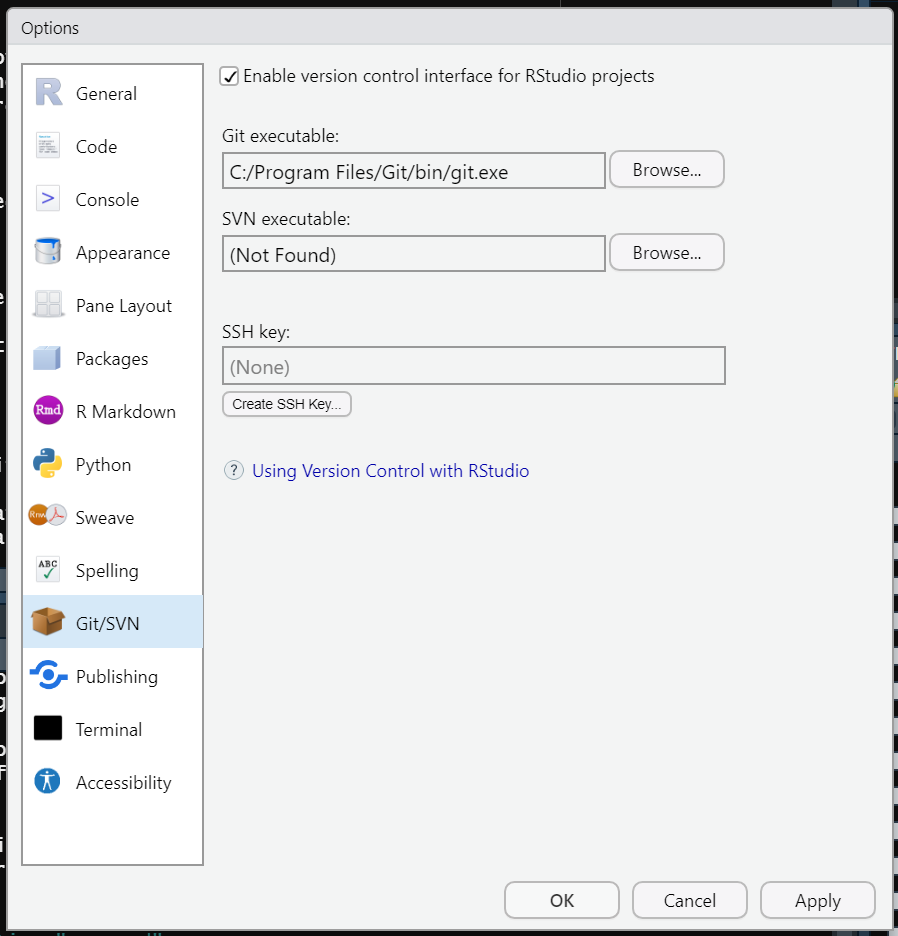
\includegraphics[width=0.64\linewidth]{images/gitdemo/gitdemo-gitRstudio-settings} \caption{Enter the path to your git executable in the git path option box}\label{fig:unnamed-chunk-1}
\end{figure}

Once you open a repository, you'll get an extra panel, named `git', in
the top right pane of R-Studio and you'll also be able to use git in the
`Terminal' tab at the bottom left (in the same place as the R console).

\begin{figure}
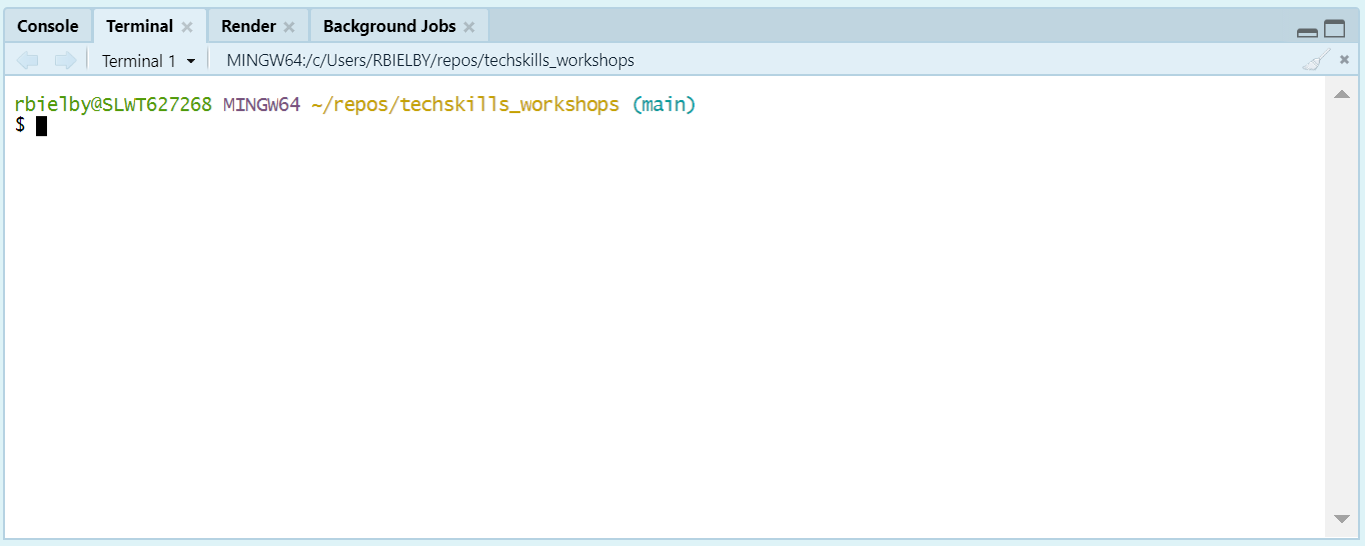
\includegraphics[width=0.56\linewidth]{images/gitdemo/gitdemo-gitRstudio-NewTerminal} \caption{The `git BASH` terminal in R-Studio}\label{fig:unnamed-chunk-2}
\end{figure}

A useful thing here if you want to use git commands in the terminal is
to switch the terminal from the default Windows Command Prompt to
\texttt{git\ BASH}. You can do this in the Terminal tab of R-Studio's
global options - just select \texttt{git\ BASH} from the `New terminal
opens with' pull down menu. Click apply and then select the Terminal tab
(next to the Console tab), click `Terminal 1' and then select `New
terminal' from the drop down menu. You should see something similar to
the terminal screenshot.

\hypertarget{working-in-teams}{%
\subsection{Working in teams}\label{working-in-teams}}

To get the most out of git and Dev Ops, you're going to need to work in
teams. We're aiming for groups of 3. Some of the tasks we'll work
through will require just one of your team to perform, whilst others
will require all of your team to perform them. If it's not clear then
ask and most importantly, communicate with each other about what you're
doing.

To help illustrate the challenges and benefits of git and Dev Ops and
how to work collectively within the same space, all the groups will be
working within the same repository. Each group will have their own
working branch (already created) with the naming format
\texttt{workshop\_group\_N}:

\begin{itemize}
\tightlist
\item
  \texttt{workshop\_group\_1}
\item
  \texttt{workshop\_group\_2}
\item
  \ldots{}
\end{itemize}

We'll need to prefix branches and tasks within the repository with
\texttt{grN\_} and group N respectively (again switching the \texttt{N}
for your group number).

By the end, you should get a good idea of how using branches can
facilitate lots of people working within the same space on the same
files independently (and where issues can occur!).

\newpage

\hypertarget{getting-started-in-dev-ops}{%
\section{Getting started in Dev Ops}\label{getting-started-in-dev-ops}}

\hypertarget{navigating-around-dev-ops}{%
\subsection{Navigating around Dev Ops}\label{navigating-around-dev-ops}}

There's a lot to Azure Dev Ops, but we're going to focus today on a
handful of key elements arund task management and repositories:

\begin{itemize}
\tightlist
\item
  Boards

  \begin{itemize}
  \tightlist
  \item
    Boards
  \end{itemize}
\item
  Repos

  \begin{itemize}
  \tightlist
  \item
    Files
  \item
    Commits
  \item
    Branches
  \item
    Pull Requests
  \end{itemize}
\end{itemize}

If you follow the link below, that should take you to our demo
repository for this workshop. Follow the link and explore the tabs on
the left of the page that are listed above.

\href{https://dfe-gov-uk.visualstudio.com/official-statistics-production/_git/workshop_devopsintro}{Azure
Dev Ops workshop\_devopsintro}

\begin{figure}
\centering
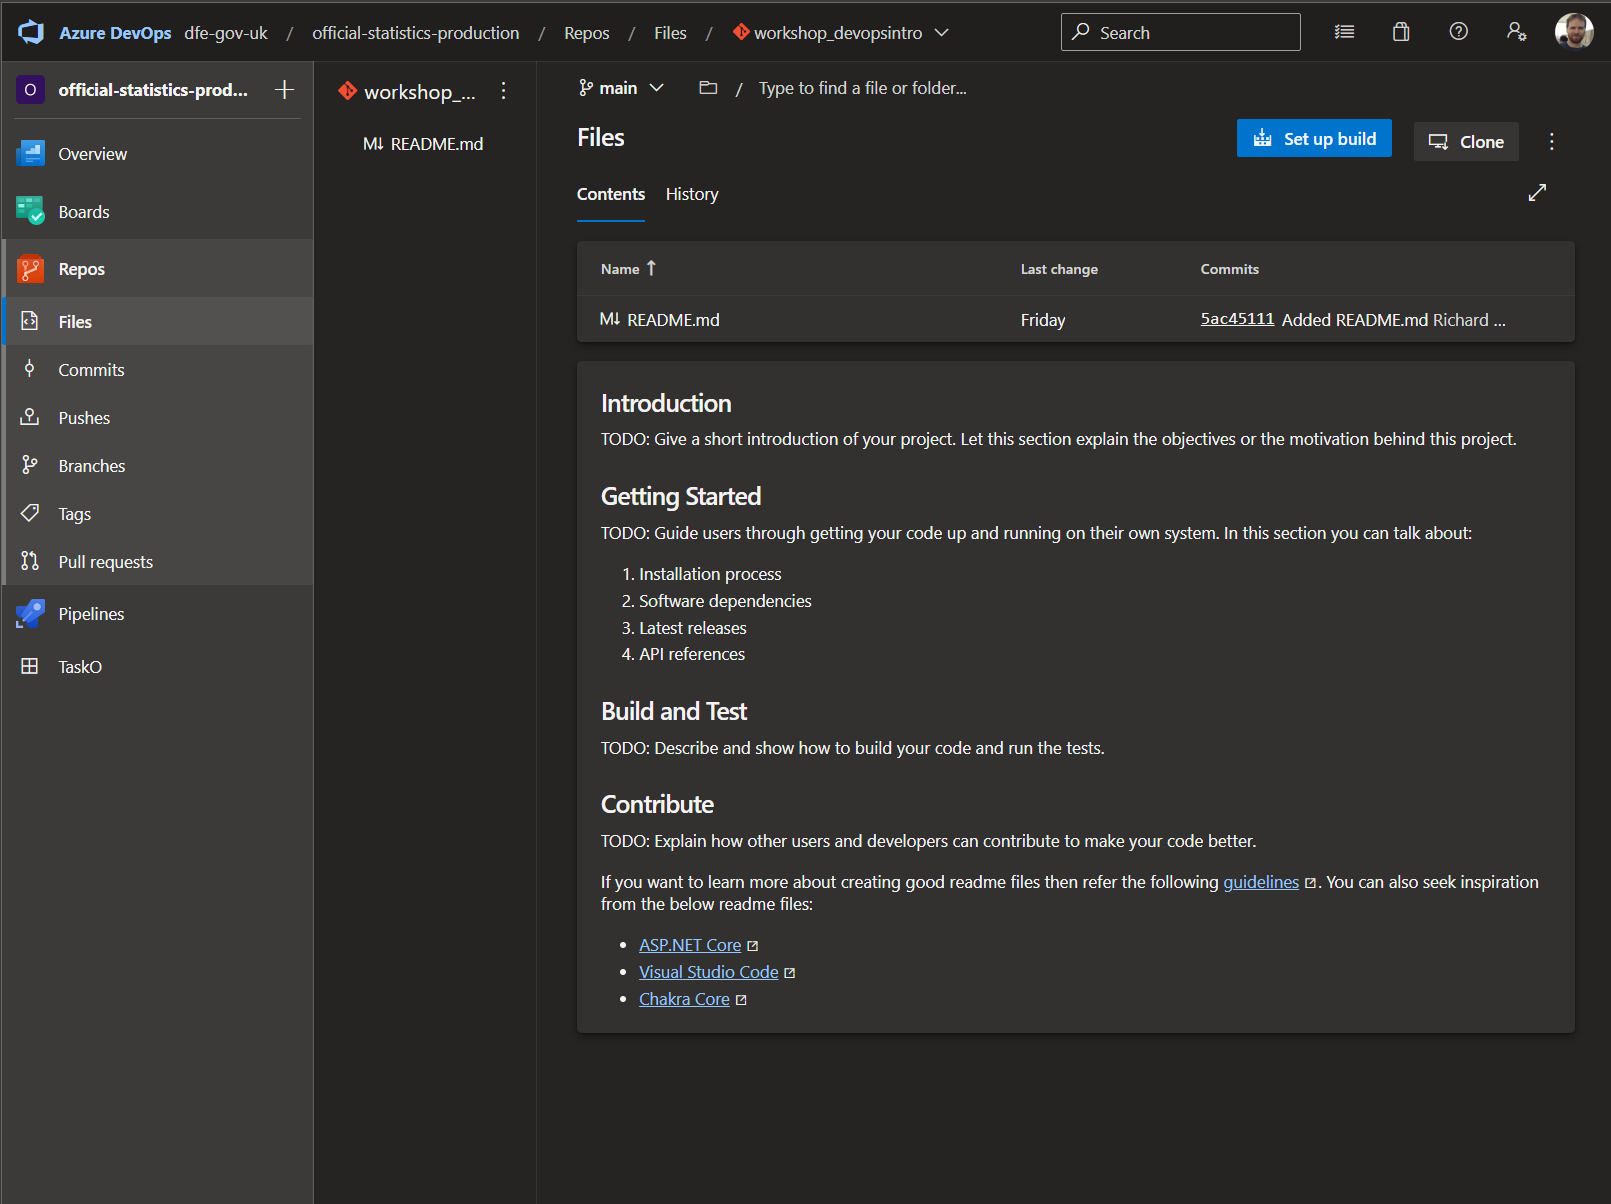
\includegraphics{images/DevOpsdemo/DevOps_repo_frontpage.PNG}
\caption{An example repository front page on Dev Ops}
\end{figure}

The key things to note at this stage is that:

\begin{itemize}
\tightlist
\item
  The Boards area contains useful project management tools for tracking
  development of your code. Today we'll just use the Kanban board style
  functionality, but there's plenty more.
\item
  The Repo area contains any repositories you have access to. You can
  navigate between repositories using the dropdown menu at the top of
  the page.
\end{itemize}

\hypertarget{whats-a-repository}{%
\subsection{What's a repository?}\label{whats-a-repository}}

A repository is a folder containing a related set of code and associated
files. So for example, it can contain your full data processing pipeline
or it could contain a dashboard app.

The repo on Dev Ops represents the central safe copy of your repository
and is called the \textbf{Remote} repository. It contains all the
history and current code of your code and should also contain at least
some associated documentation (primarily in the form of the Readme.md
file).

You and your team can also have as many copies (or clones) of the
repository on your workstations. These are the \textbf{Local}
repositories. Any updates that you and your team make to the files in
your local copies of the repository should be synced to the remote
repository at regular intervals, such that all team members can access
the latest versions of the files.

\hypertarget{cloning-the-repository-to-your-local-machine}{%
\subsection{Cloning the repository to your local
machine}\label{cloning-the-repository-to-your-local-machine}}

Cloning the repository refers to creating a copy of the remote
repository (i.e.~the copy on GitHub or Dev Ops) on the disk on your
local machine (i.e.~your DfE laptop). For an R project, there are two
basic options to choose from for doing this:

\begin{itemize}
\tightlist
\item
  using the R-Studio new project wizard, or
\item
  using \texttt{git\ BASH}.
\end{itemize}

We'd recommend trying the different options across your working group.

Before starting either option, you'll need to copy the repo url from Dev
Ops. To do this, open up the repo front page in Dev Ops (you can use the
link from earlier) and click the grey \textbf{Clone} button near the top
right of the page. Make sure HTTPS is selected and then click the copy
button to grab the url.

\hypertarget{cloning-in-git-bash}{%
\subsubsection{\texorpdfstring{Cloning in
\texttt{git\ BASH}}{Cloning in git BASH}}\label{cloning-in-git-bash}}

You can open up a \texttt{git\ BASH} terminal, by typing
\texttt{git\ BASH} in the Windows search bar and select
\texttt{git\ BASH} when it comes up. With a terminal, you can interact
with it just by typing, similar to working in the R console in RStudio.
First let's make a directory in which to store our repositories:

\begin{verbatim}
    mkdir repos
\end{verbatim}

We can then move into the directory we just created using:

\begin{verbatim}
    cd repos
\end{verbatim}

Now grab the repo url and replace
\texttt{\textless{}repo\_url\textgreater{}} in the next command with the
actual url from Dev Ops:

\begin{verbatim}
    git clone <repo_url>
\end{verbatim}

You should get some messages letting you know git is connecting to the
server and cloning the repository and it should look something like the
figure below.

\begin{figure}
\includegraphics[width=0.6\linewidth]{images/gitdemo/gitdemo-terminal_clone} \caption{Cloning a repository in git BASH}\label{fig:unnamed-chunk-3}
\end{figure}

If all went well, you'll now have a complete copy of the repository on
your laptop. To open the repository in RStudio, start up RStudio and
select Open project. In the file explorer window that opens up, type
\texttt{C:\textbackslash{}Users\textbackslash{}} and hit enter (see the
screenshot below) and then open up your home folder.

\begin{figure}
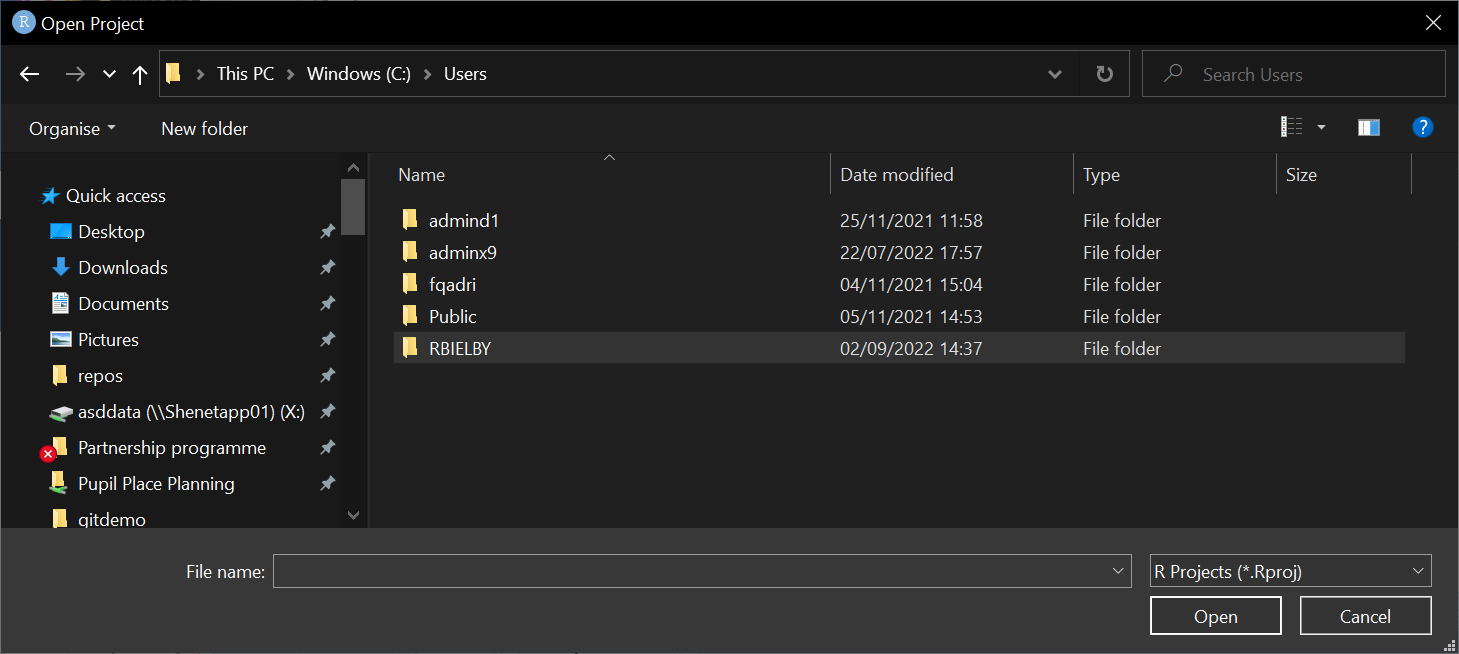
\includegraphics[width=0.6\linewidth]{images/gitdemo/gitdemo-RStudio_OpenProj} \caption{Open a cloned project in RStudio}\label{fig:unnamed-chunk-4}
\end{figure}

Then navigate into \texttt{repos} and the repository folder. The full
path should be something along the lines of:

\begin{quote}
\texttt{This\ PC\ \textgreater{}\ Windows\ (C:)\ \textgreater{}\ Users\ \textgreater{}\ \textless{}USERNAME\textgreater{}\ \textgreater{}\ repos\ \textgreater{}\ \textless{}REPONAME\textgreater{}}
\end{quote}

Select the R project file and select open.

\begin{figure}
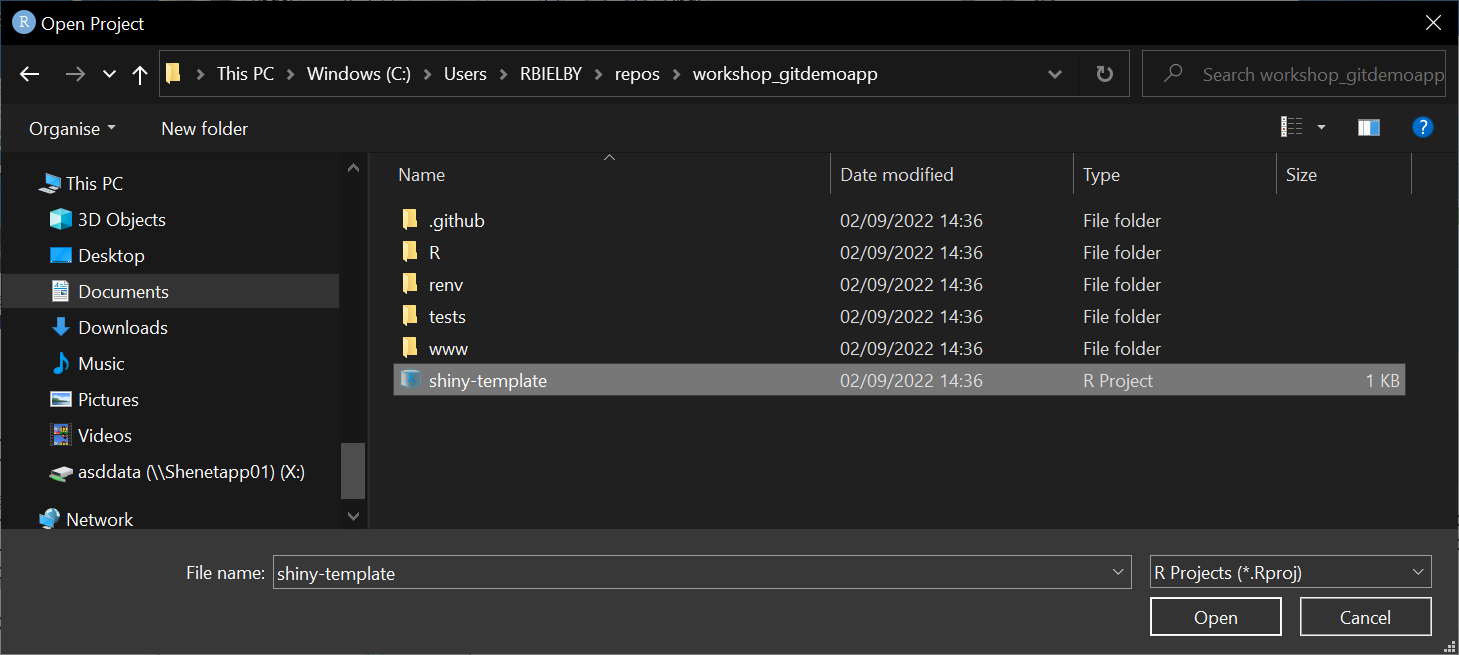
\includegraphics[width=0.6\linewidth]{images/gitdemo/gitdemo-RStudio_OpenProj_fullpath} \caption{Open a cloned project in RStudio}\label{fig:unnamed-chunk-5}
\end{figure}

\hypertarget{cloning-using-the-rstudio-wizard}{%
\subsubsection{Cloning using the RStudio
wizard}\label{cloning-using-the-rstudio-wizard}}

If that looks like a bit too much text based effort, RStudio offers a
way to clone a repository with it's New project wizard. To do this
navigate the menu bar to \textbf{File \textgreater{} New
Project\ldots{}}, select \textbf{Version Control} and then Git. This
opens up a dialogue box to enter the repository url and select where to
save it. As with the git BASH version, copy and paste your remote repo
URL here and set a directory where you want it saved on your laptop.

\begin{figure}
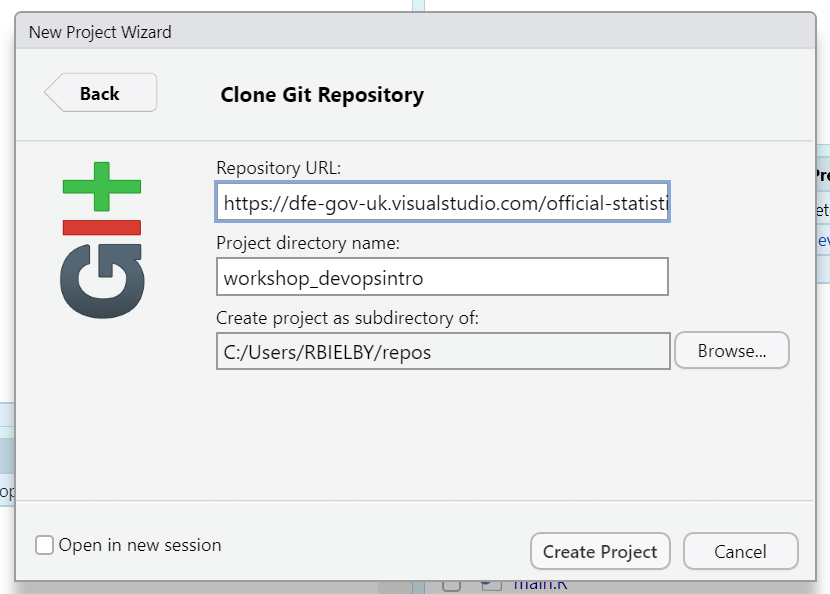
\includegraphics[width=0.6\linewidth]{images/DevOpsdemo/DevOps_RStudio_clonerepo} \caption{Clone a project using the RStudio git wizard}\label{fig:unnamed-chunk-6}
\end{figure}

\hypertarget{a-note-on-local-repository-clones-and-onedrive}{%
\paragraph{A note on local repository clones and
OneDrive}\label{a-note-on-local-repository-clones-and-onedrive}}

\begin{quote}
Note that saving a repository within your OneDrive folder structure can
cause some awkward issues. If you use git to perform version control on
a repository saved within a OneDrive folder, you may start receiving
warning messages that large numbers of files have been removed from
OneDrive. In addtion, it can put a heavy burden on your internet
connection as OneDrive tries to keep up with changes to the files
managed by git. Best practice therefore is to store your repositories
somewhere outside your OneDrive file structure. We recommend creating a
\texttt{repos} directory within your base User directory
(i.e.~\texttt{C:\textbackslash{}Users\textbackslash{}\textless{}USERNAME\textgreater{}\textbackslash{}repos\textbackslash{}}.
Windows sometimes tries to make it awkward for you to navigate to places
on your laptop outside of the OneDrive folders, so a useful tip is to
add your \texttt{repos} folder to your Quick access list in File
Explorer.
\end{quote}

\hypertarget{using-dev-ops-boards}{%
\subsection{Using Dev Ops Boards}\label{using-dev-ops-boards}}

We're going to work through a demo of tidying up some data and running a
quick QA on it.

To start with, we'll create some tasks on the Kanban Board in Dev Ops.
The tasks to create are (note that including your group number in the
titles will make things easier further down the line):

\begin{itemize}
\tightlist
\item
  Group N: \protect\hyperlink{tidying-the-data}{Tidying the data}
\item
  Group N: \protect\hyperlink{creating-the-wide-data-plot}{Creating the
  wide data plot}
\item
  Group N: \protect\hyperlink{creating-the-tidy-data-plot}{Creating the
  tidy data plot}
\end{itemize}

Go to the \emph{Boards} \textgreater{} \emph{Boards} tab on Dev Ops and
make sure you're in the right board, i.e.~workshop\_devopsintro\_N. Now
create tasks for each of these using the New item button.

\hypertarget{summary}{%
\subsection{Summary}\label{summary}}

In this section, we've had a quick look around Dev Ops and the remote
repository, cloning it to your local drive (using both the BASH terminal
and the RStudio wizard) and creating and assigning tasks on the Dev Ops
Boards area.

In the next section, we'll cover some of the basics of using git to log
changes to your code and sync them between the remote repo and local
copies. If you open up one of the tasks, you'll see you can add
descriptions, comments, tags, priorities and story points (effectively
an estimate of the effort or time required) among other things. We can
leave those for the purpose of this demo and for now decide who's going
to do what and drag each task into the Active column. Note that whoever
drags a given task across will automatically be assigned as the person
working on that task. If that's not the right person, then click on the
name and select who should be doing it.

We'll take a break from Dev Ops now and move on to taking a look at
using git.

\newpage

\hypertarget{basics-of-git}{%
\section{Basics of git}\label{basics-of-git}}

We'll now take a look at updating repositories using some simple
processing and QA code as an example.

\hypertarget{the-git-log}{%
\subsection{The git log}\label{the-git-log}}

In order to move quickly between different versions of files and code,
git is built around indexing and a log file that track the changes in a
repository. To view the log of any repository, we can simply go into
that repository and run the command \texttt{git\ log} from the BASH
terminal. Here's a minimal example on a fresh repsoitory:

\begin{center}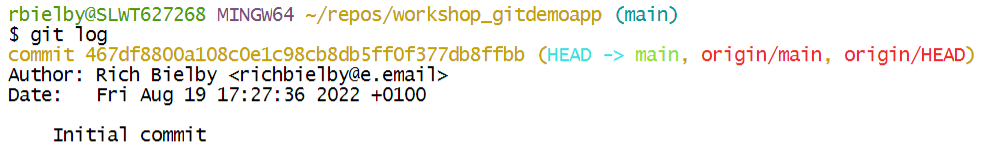
\includegraphics[width=0.8\linewidth]{images/gitdemo/gitdemo-gitlog-1} \end{center}

The log shows all ``commits'' that have been made to the repository.
We'll go into making commits in the next section.

\hypertarget{git-bash-versus-the-r-studio-git-panel}{%
\subsection{\texorpdfstring{\texttt{git\ bash} versus the
\emph{R-Studio} git
panel}{git bash versus the R-Studio git panel}}\label{git-bash-versus-the-r-studio-git-panel}}

\begin{figure}

{\centering 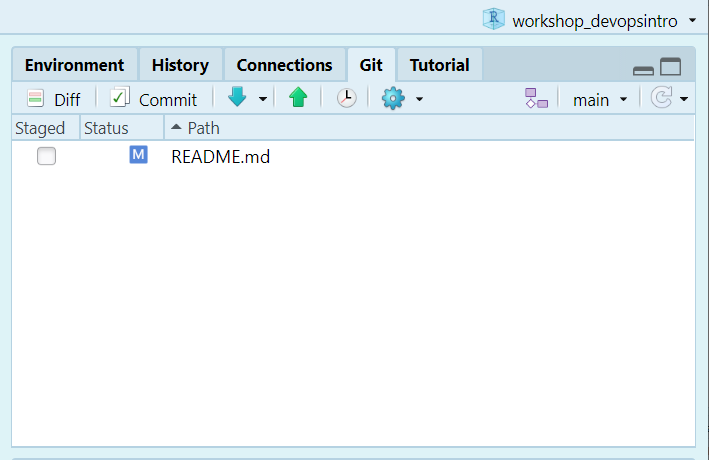
\includegraphics[width=0.5\linewidth]{images/gitdemo/gitDemo-RStudio_gitinterface} 

}

\caption{The *R-Studio* git panel provides all the common day to day git commands such as Stage/Add, Commit, Push and Pull, switch branches, view history.}\label{fig:unnamed-chunk-8}
\end{figure}

\begin{figure}

{\centering 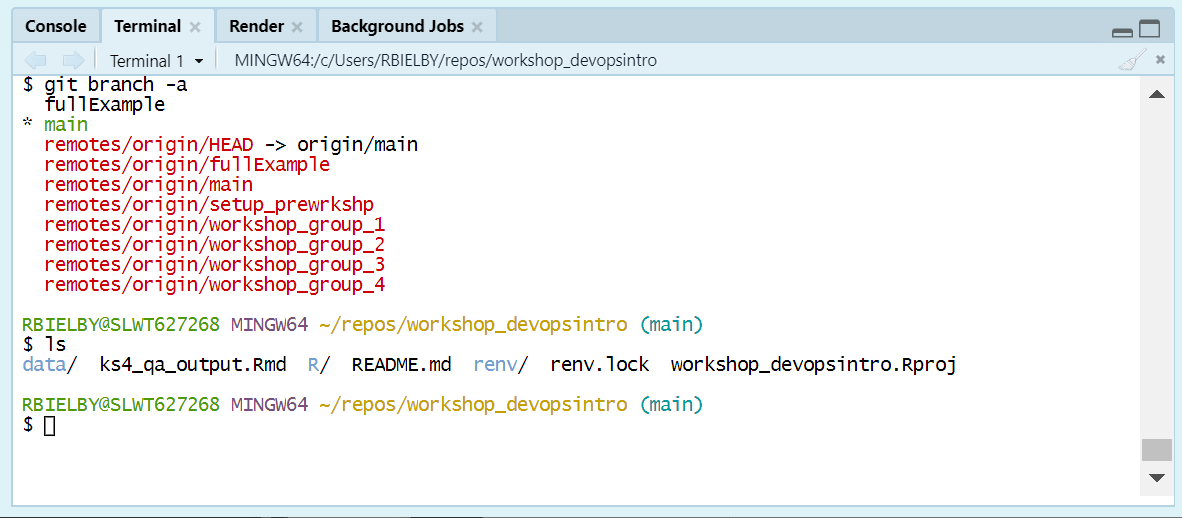
\includegraphics[width=0.5\linewidth]{images/gitdemo/gitDemo-RStudio_gitterminal} 

}

\caption{The *R-Studio* git bash terminal provides access to all git functionality via a command line interface.}\label{fig:unnamed-chunk-9}
\end{figure}

There are two main ways you can run git commands within R-Studio, either
using the \texttt{git\ bash} terminal or the \emph{R-Studio} git panel
Each offers some advantages, but the main ones are that
\texttt{git\ bash} offers the full range of tools for controlling your
repository, whilst the \emph{R-Studio} git panel offers the most common
basic commands but with a simpler (and usually quicker) interface. We'll
use both in this workshop.

\hypertarget{branches}{%
\subsection{Branches}\label{branches}}

One of the most important elements of using \texttt{git} is
\textbf{branches}. These provide a method to keep multiple different
copies of your code in a single repository. This is usually intended to
maintain a working base copy alongside one or many development branches
with new features, updates or bugfixes.

In this workshop, we've created a branch for each team, so you need to
start by switching to the branch for your group - one of
workshop\_group\_1, workshop\_group\_2, workshop\_group\_3 etc. As in
most cases here, you can use either the RStudio git panel or
\texttt{git\ bash} to switch branches.

\hypertarget{switching-branches-in-git-bash}{%
\subsubsection{\texorpdfstring{Switching branches in
\texttt{git\ bash}}{Switching branches in git bash}}\label{switching-branches-in-git-bash}}

In \texttt{git\ bash}, you can change branches using either the
\texttt{switch} or \texttt{checkout} command. Go to the bash terminal in
R-Studio and enter the command:

\texttt{git\ checkout\ workshop\_group\_1}

Updating the number to your group number. To switch back to main, you
can simply use:

\texttt{git\ checkout\ main}

\hypertarget{switching-branches-in-the-r-studio-git-panel}{%
\subsubsection{\texorpdfstring{Switching branches in the \emph{R-Studio}
git
panel}{Switching branches in the R-Studio git panel}}\label{switching-branches-in-the-r-studio-git-panel}}

In the git panel, the name of the current branch is given next to the
purple create branch symbol. Click on the name of the current branch
(which should be \emph{main} at present) and a drop down list will
appear. Select your group's branch from this list and R-Studio will
automatically switch to that branch. Anything you add and commit to the
repository will now be written to the branch you've selected and not
\emph{main}.

\hypertarget{adding-commiting-and-pushing}{%
\subsection{Adding, commiting and
pushing}\label{adding-commiting-and-pushing}}

To have something to work with, we need some data. There should be a
data folder in the repository already, so all we need to do is grab some
data and save it there. For this workshop, we'll use a file from a
publication on Explore Education Statistics.

\emph{For this section, just one of your group should run through the
following steps in your group's branch:}

Go to
\href{https://explore-education-statistics.service.gov.uk/data-catalogue/key-stage-4-performance-revised/2020-21}{key
stage 4 performance publication} and download the \textbf{KS4 subject
timeseries data (csv, 364 Kb)} file, extract the data csv file
(\emph{2021\_subject\_timeseries\_data.csv}) and save it into the repo's
data folder (you can just use the normal Windows File Explorer to do
this).

Now to add this to the git tracking: run the following commands:

\begin{verbatim}
  git add .
\end{verbatim}

This searches the repo for any files that have been modified since the
last commit and creates a log of the changes. If you want to check that
the command has worked, then you can type \texttt{git\ status} or
\texttt{git\ st} and you'll get a summary of files that have been staged
and are ready to commit.

\begin{verbatim}
  git commit -m "Added data file into repository."
\end{verbatim}

This adds an entry on to the log, updating it with the file changes that
you've just made. Note that the text after the \texttt{-m} is a comment
used to describe the changes to make it easier for someone looking back
from the log to see what changes have happened. Those are the two key
steps for tracking changes to the files and folders in your repository.

Now we'll add in some simple code to read in the file. Create a script
in the repository's root directory called \texttt{main.R}. The add the
following code to it:

\begin{verbatim}
dfKS4 <- read.csv('data/2021_subject_timeseries_data.csv')
colnames(dfKS4)[1] <- "time_period"
\end{verbatim}

Let's do a quick commit to log that change. In the terminal run
\texttt{git\ add\ .} and
\texttt{git\ commit\ -m\ "Added\ new\ data\ and\ reading\ it\ in."}.

If we now run \texttt{git\ log} again, we get something along the lines
of:

\begin{center}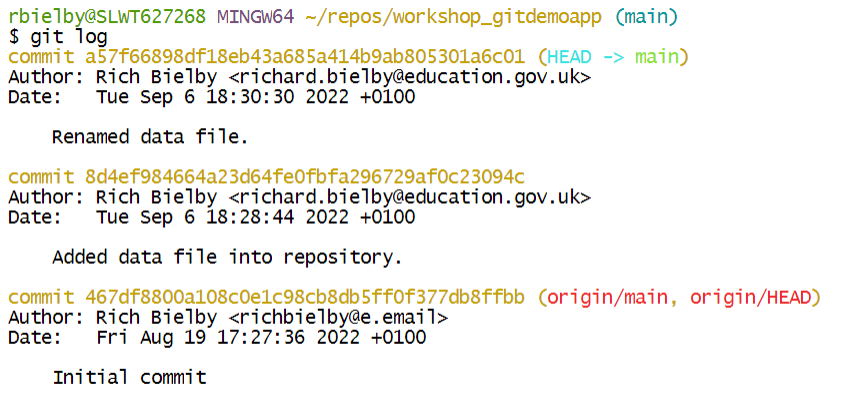
\includegraphics[width=0.8\linewidth]{images/gitdemo/gitdemo-gitlog-2} \end{center}

Here we can see, in reverse order, the commits that have been made, who
made them, when they made them, and the messages that have been recorded
with them.

Finally, it's important to note that what we've done so far is only
being applied to the local copy of the repository (i.e.~the copy on your
laptop). To apply your changes to the remote repository (i.e.~on GitHub
or Dev Ops), you need to ``push'' the changes. This can be done a couple
of different ways: a) in the terminal type \texttt{git\ push} or b) on
the toolbar in the \emph{R-Studio} git panel press the green up button!
Once you've done this, open up a browser and go to your remote
repository on Dev Ops and, once you've switched on to your branch, you
should now see the data file stored there. You should also see that it's
not been added on to the main branch.

\hypertarget{pulling-from-the-remote-repository}{%
\subsection{Pulling from the remote
repository}\label{pulling-from-the-remote-repository}}

Now that you've made changes, the rest of your team need to update their
own local copies of the repository with your updates by pulling from the
remote. Similarly to pushing, they can do this by either a) typing
\texttt{git\ pull} in the BASH terminal or b) pressing the down arrow in
the toolbar of the git panel in \emph{R-Studio}.

\hypertarget{summary-of-git-basics}{%
\subsection{Summary of git basics}\label{summary-of-git-basics}}

We've quickly tried out a quick cycle of adding and committing, which is
used to log changes into the local repository and then we've pushed and
pulled to and from the remote repository and local copies on different
laptops. The table below gives a summary of the relevant commands in the
BASH terminal and the corresponding buttons in the RStudio git panel.

\begin{longtable}[]{@{}
  >{\raggedright\arraybackslash}p{(\columnwidth - 4\tabcolsep) * \real{0.0968}}
  >{\raggedright\arraybackslash}p{(\columnwidth - 4\tabcolsep) * \real{0.3763}}
  >{\raggedright\arraybackslash}p{(\columnwidth - 4\tabcolsep) * \real{0.5269}}@{}}
\toprule()
\begin{minipage}[b]{\linewidth}\raggedright
Process
\end{minipage} & \begin{minipage}[b]{\linewidth}\raggedright
git BASH
\end{minipage} & \begin{minipage}[b]{\linewidth}\raggedright
RStudio git panel
\end{minipage} \\
\midrule()
\endhead
Add & \texttt{git\ add\ .} & Stage using tickbox next to each modified
file. \\
Commit & \texttt{git\ commit\ -m\ "Commit\ message."} & ``Commit''
button in toolbar. \\
Push & \texttt{git\ push} & Green up arrown in toolbar. \\
Pull & \texttt{git\ pull} & Blue down arrow in toolbar. \\
View the log & \texttt{git\ log} & Clock icon in toolbar. \\
\bottomrule()
\end{longtable}

\newpage

\hypertarget{working-collaboratively-with-git}{%
\section{Working collaboratively with
git}\label{working-collaboratively-with-git}}

Git only really makes proper sense once multiple people start working on
a project collaboratively. Solo working, git is useful for version
control and syncing your work to a remote repository site like Dev Ops
and GitHub, but may not feel like it offers all that much more beyond
that. Once we start working collaboratively however, the benefits of
using git (alongside GitHub or Dev Ops) become more apparent. We'll now
look further into this with some worked examples.

\hypertarget{branches-and-splitting-tasks}{%
\subsection{Branches and splitting
tasks}\label{branches-and-splitting-tasks}}

\hypertarget{task-management}{%
\subsubsection{Task management}\label{task-management}}

One useful management tool that we can use from Dev Ops is the
\emph{Boards} area. Here we can create individual tasks, assign them to
team member and then create new \textbf{branches} from those tasks. You
can think of \textbf{branches} as self contained copies of the
repository that can contain complementary or conflicting differences
with all other \textbf{branches} in the repository. These allow you to
work on different multiple tasks on your code independently of any other
changes you might be making. Bringing these different \textbf{branches}
or tasks together is then managed using \textbf{merges} or \textbf{pull
requests} (PRs).

We'll demonstrate this by performing 3 related tasks on 3 different
branches. Each task should be done by only one of your group, so split
the following 3 tasks between your group and each follow the relevant
instructions in the subsections below:

\begin{itemize}
\tightlist
\item
  1a) Tidying the data
\item
  1b) Creating the wide data plot
\item
  1c) Creating the tidy data plot
\end{itemize}

Once you've decided who's doing what, each of you should jump to the
relevant section below. And remember that you're not working in
independent silos here, what you do can impact what other people are
doing so communication needs to happen along the way.

\hypertarget{tidying-the-data}{%
\paragraph{Tidying the data}\label{tidying-the-data}}

Start the task by going to your Dev Ops board and click on the options
for the Tidying data task. Select \textbf{Create new branch} from the
drop down menu that appears over the task. You'll get a pop-up dialogue
box with some options about your new branch. Give the new branch a name
(e.g.~\texttt{grN\_task1}), make sure it's based on your group's branch
(\texttt{workshop\_group\_N}) in the \texttt{workshop\_devopsintro} repo
and then click \textbf{Create branch}.

\begin{center}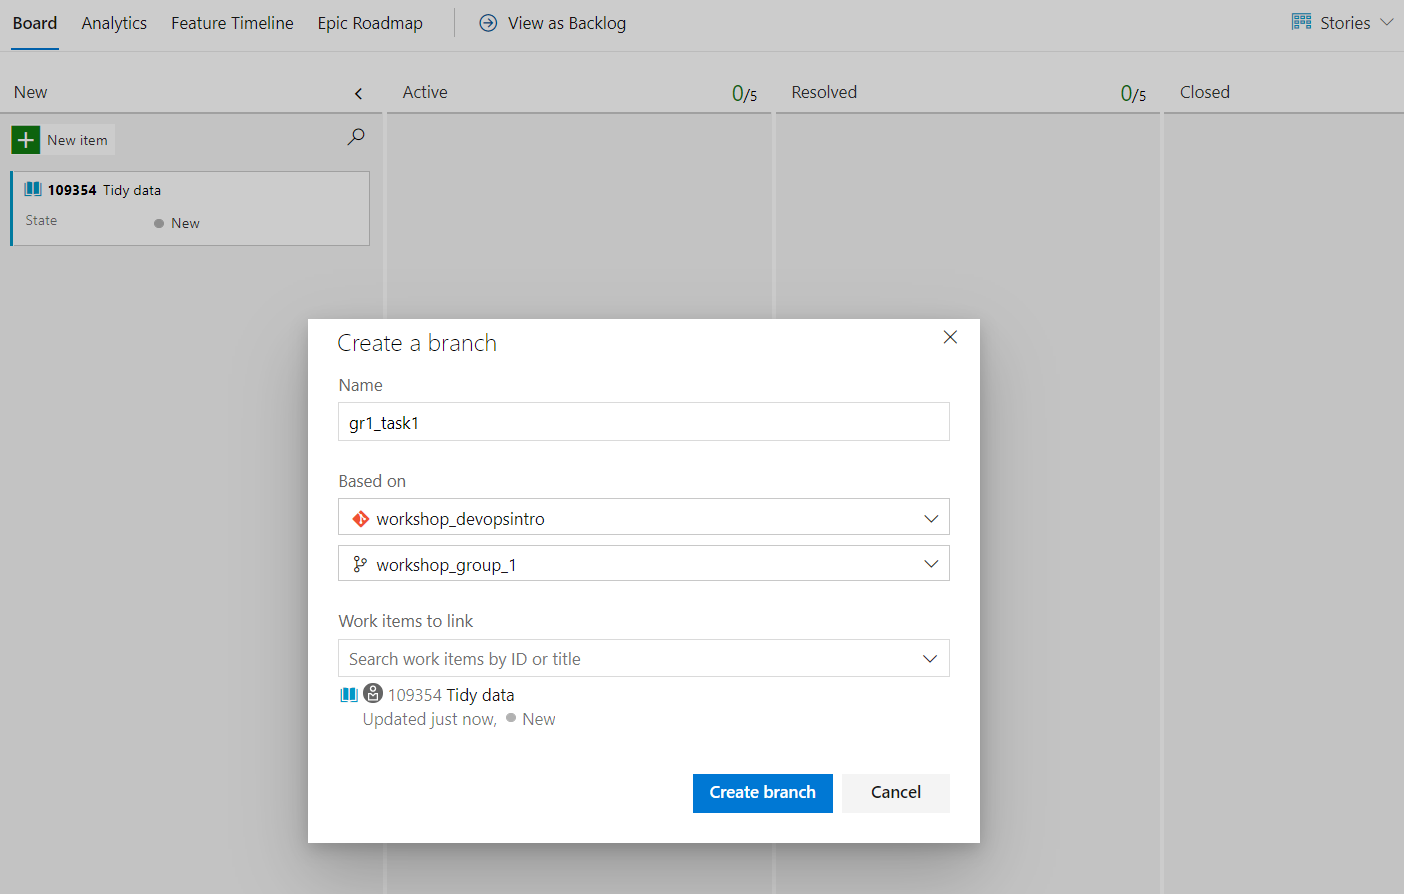
\includegraphics[width=0.8\linewidth]{images/DevOpsdemo/DevOps_Boards_newbranch} \end{center}

You'll now have a new branch in your remote repo that's identical to
your groups working branch. To access that branch in your local repo,
you just need to perform a pull (i.e.~\texttt{git\ pull} in the
\texttt{bash} terminal or the down arrow in the R-Studio git panel) and
then switch branches (\texttt{git\ switch\ grN\_task1} in \texttt{bash}
or select from the drop down menu in the git panel).

Now to make the edits. Copy and paste the following code into the script
\texttt{R/utils.R}:

\begin{verbatim}
tidy_subject_timeseries <- function(dfin){
  # Pivot long and then update the string values in the new filter column.
  dftidied <- dfin  %>%
    pivot_longer(!c(time_period,time_identifier,geographic_level,
                    country_code,country_name,version,characteristic_gender,
                    subject,entries),
                 names_to="level",
                 values_to="percentage_pupils")
  colnames(dftidied) <- gsub("characteristic_","",colnames(dftidied))
  return(dftidied)
}
\end{verbatim}

And then go back to \texttt{main.R} and add the lines:

\begin{verbatim}
library(tidyr)
library(dplyr)
source('R/utils.R')
dfKS4tidied <- tidy_subject_timeseries(dfKS4)
\end{verbatim}

At this point you could try sourcing \texttt{main.R} in the R console
and that should create the data frame \texttt{dftidied} (and hopefully
not produce any errors!).

Once you're happy, then run another
\texttt{add}/\texttt{commit}/\texttt{push} cycle and flag to your team
that you've finished the code to read in the data. Then scroll down this
guide to the \protect\hyperlink{merging-and-pull-requests}{merging and
pull requests} section.

\hypertarget{creating-the-wide-data-plot}{%
\paragraph{Creating the wide data
plot}\label{creating-the-wide-data-plot}}

Whilst the first task adds in some data, reads it in and does some
processing, this task builds a quick chart based on the data.

Create a new branch within R-Studio. To do this, first make sure that
you're in your groups branch (i.e.~\texttt{workshop\_group\_N}) and then
you can either a) use the command \texttt{git\ checkout\ -b\ grN\_task2}
(changing the N to your group number) and push to the remote
(\texttt{git\ push}) or click the purple new branch button in the
R-Studio git panel (see the image below).

\begin{center}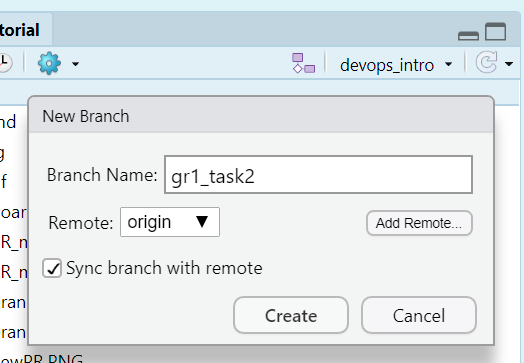
\includegraphics[width=0.92\linewidth]{images/DevOpsdemo/DevOps_RStudio_newbranch} \end{center}

We want to track this branch with the associated task in Dev Ops Boards,
so go to the card you made for task 2 on your group's board. Move it to
the \textbf{Active} column and then open up the task to edit. On the
right hand side of the dialogue box, you can link your branch to this
task under \textbf{Development}. Click \textbf{Add link} and in the next
dialogue box find and select your new branch from the branch drop down
menu (as shown in the screenshot). Click Ok to complete the link. Then
you should see your branch listed under \textbf{Development} (note the
option to create a Pull request, which you can use later on when we
merge this branch in to the rest of the development).

\begin{center}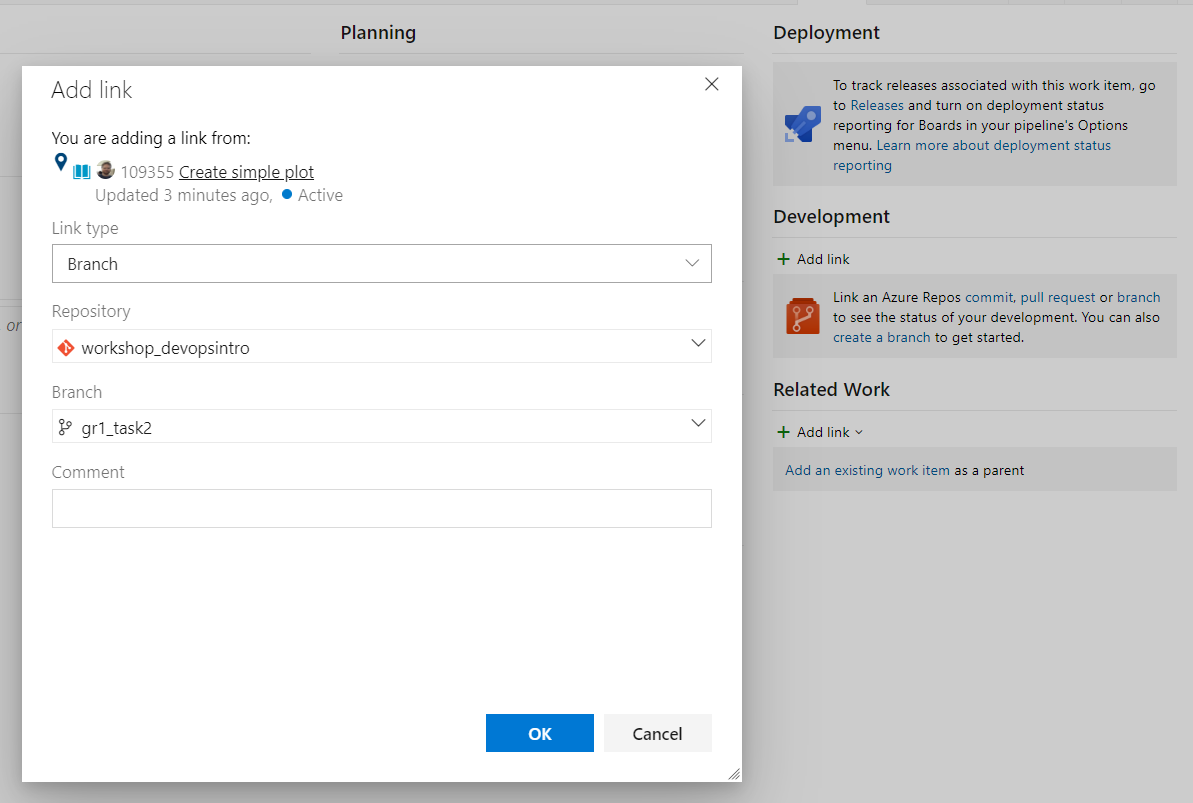
\includegraphics[width=0.82\linewidth]{images/DevOpsdemo/DevOps_Boards_linkbranch} \end{center}

Now to make the changes. Head back to R-Studio and add the following
lines of code to \texttt{R/plots.R} in your local copy of the
repository:

\begin{verbatim}
plot_ACrange <- function(df){
  dfplot <- df %>% filter(time_period>=201920,
                             !X94AstarC %in% c('z',':','x'),
                             grepl('Studies',subject)) %>% 
    select(time_period,characteristic_gender,entries,subject,X94AstarC) %>%
    mutate(entries=as.numeric(entries)/1.e3,
           X94AstarC=as.numeric(X94AstarC))
  df1 <- dfplot %>% filter(time_period==202021,characteristic_gender=='Total')
  plot(df1$entries,df1$X94AstarC)
}
\end{verbatim}

And the following to \texttt{main.R}:

\begin{verbatim}
library(dplyr)
source('R/plots.R')
plot_ACrange(dfKS4)
\end{verbatim}

And that should be it for this task. All that's left is to commit and
push your changes. If you've got a preferred way already to perform
commits, then go for it. If not then let's use the RStudio git panel.

\begin{figure}

{\centering \includegraphics[width=0.64\linewidth]{images/gitdemo/gitdemo-RStudio-gitpanel} 

}

\caption{Staging files in the RStudio git panel.}\label{fig:unnamed-chunk-14}
\end{figure}

Firstly click on the git tab in the top right of RStudio to show the git
panel (see the screenshot below). Next click the tickboxes next to the
files with changes (i.e.~these should be server.R and
R/dashboards\_panels.R) to \textbf{stage} (aka \textbf{add}) the files.
Now click \textbf{commit}, add a commit message in the relavent text box
and then hit \textbf{commit} in the bottom right corner of the window.

Assuming that all went through without any issues, you can now press the
green up arrow in the git panel to \textbf{push} your changes to the
remote repository on Dev Ops

Flag to your team that you've finished the code to read in the data.
Then scroll down this guide to the
\protect\hyperlink{merging-and-pull-requests}{merging and pull requests}
section.

\hypertarget{creating-the-tidy-data-plot}{%
\paragraph{Creating the tidy data
plot}\label{creating-the-tidy-data-plot}}

Start by creating a new branch in Dev Ops. Navigate to the files panel
of the repo on Dev Ops and click the branch drop down menu. Select your
groups working branch (\texttt{working\_group\_N}). Click the drop down
again and now select \textbf{+ New branch}. You'll get a pop-up dialogue
box that looks like the image below. Fill in a name for the new branch
and make sure your groups working branch is selected in the
\textbf{Based on} selection box. You can also link your task to this new
branch by selecting it in the \textbf{Work items to link} selection box.
Once you've done that, quickly go to your group's board and have a look
at the task 3 card. If you haven't done so already, drag and drop the
card into the Active column (you should then see that you automatically
get asigned to the task in Dev Ops).

\begin{center}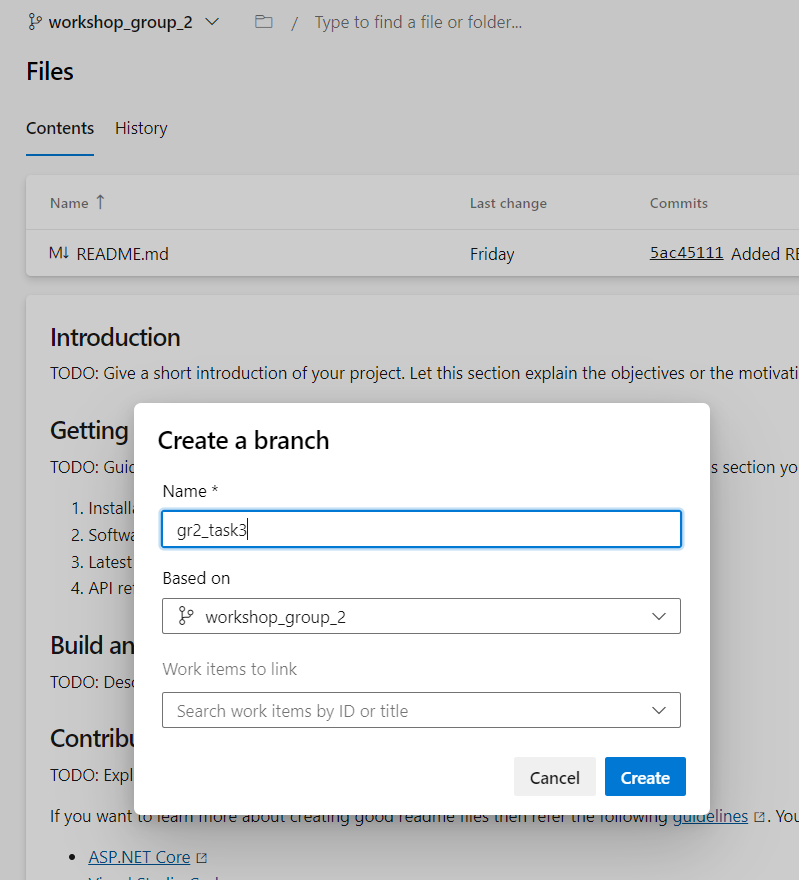
\includegraphics[width=0.64\linewidth]{images/DevOpsdemo/DevOps_Repo_newbranch} \end{center}

Now head to R-Studio, perform a pull (\texttt{git\ pull} in the terminal
or the green down arrow in the git panel) and then switch to your new
branch.

Then go ahead and add the following lines of code to \texttt{R/plots.R}
in your local copy of the repository:

\begin{verbatim}
plot_ACrange_tidy <- function(dftidy){
  df <- dftidy %>% filter(time_period>=201920,level=='X94AstarC',
                          !percentage_pupils %in% c('z',':','x'),
                          grepl('Studies',subject)) %>%
    mutate(time_period = as.character(time_period),
           entries=as.numeric(entries)/1.e3,
           percentage_pupils=as.numeric(percentage_pupils)) %>%
    mutate(achieved = as.numeric(percentage_pupils)/100.*entries)
  ggplot(df,aes(x = entries,
                y=percentage_pupils,group=time_period,color=subject)) +
    geom_point() +
    facet_grid(time_period ~ gender)
}
\end{verbatim}

And the following to \texttt{main.R}:

\begin{verbatim}
library(dplyr)
library(ggplot2)
source('R/plots.R')
plot_ACrange_tidy(dfKS4tidied)
\end{verbatim}

And that should be it for this task. All that's left is to commit and
push your changes. If you've got a preferred way already to perform
commits, then go for it. If not then let's use the RStudio git panel.

\begin{figure}

{\centering \includegraphics[width=0.64\linewidth]{images/gitdemo/gitdemo-RStudio-gitpanel} 

}

\caption{Staging files in the RStudio git panel.}\label{fig:unnamed-chunk-16}
\end{figure}

Firstly click on the git tab in the top right of RStudio to show the git
panel (see the screenshot below). Next click the tickboxes next to the
files with changes (i.e.~these should be server.R and
R/dashboards\_panels.R) to \textbf{stage} (aka \textbf{add}) the files.
Now click \textbf{commit}, add a commit message in the relavent text box
and then hit \textbf{commit} in the bottom right corner of the window.

Assuming that all went through without any issues, you can now press the
green up arrow in the git panel to \textbf{push} your changes to the
remote repository on GitHub.

Flag to your team that you've finished the code to read in the data.
Then scroll down this guide to the
\protect\hyperlink{merging-and-pull-requests}{merging and pull requests}
section.

\hypertarget{merging-and-pull-requests}{%
\subsection{Merging and pull requests}\label{merging-and-pull-requests}}

As part of using branches within git, you'll reach the point where you
need to merge two branches together. This can be done with a git command
from the \texttt{BASH} terminal, but usually it's more helpful to
perform merges using a \emph{Pull Request (PR)} in Dev Ops or GitHub.
The difference between a merge and a pull request is basically that a
pull request is a way to run a merge from Dev Ops or GitHub which
provides some useful tracking tools to help you clearly understand and
communicate what is happening as part of a given merge. Some key things
the pull requests offer are:

\begin{itemize}
\tightlist
\item
  user documentation of changes;
\item
  quick look diff/overview of changes made to files on the branch being
  merged;
\item
  run automated tests;
\item
  ability for collaborators to review your code;
\item
  control of merge conflicts;
\item
  final sign-off from collaborators;
\item
  complete a merge.
\end{itemize}

We'll start though by trying a basic \texttt{git\ merge} from the
terminal without these features offered by pull requests.

\hypertarget{git-merge-and-a-simple-merge-conflict}{%
\subsubsection{\texorpdfstring{\texttt{git\ merge} (and a simple merge
conflict)}{git merge (and a simple merge conflict)}}\label{git-merge-and-a-simple-merge-conflict}}

As we've left things, the code for task 1 and task 2 both should work
without errors. However, the code for task 3 (plotting from the tidied
data frame) requires the code from task 1 (which produces the tided data
frame) to be able to run. To get it running, we're going to merge the
branch for task 1 into the branch for task 3. To do this, \emph{one of
your team} should switch into the branch for task 3
(e.g.~\texttt{git\ switch\ task3}) and then run the following command:

\begin{verbatim}
   git merge task1
\end{verbatim}

This will attempt to merge the task1 branch into the task3 branch.
However, this will produce a merge conflict and the merge will not
complete. If you now look at the script \texttt{main.R}, it should now
look something like the following:

\begin{verbatim}
   dfKS4 <- read.csv('data/2021_subject_timeseries_data.csv')
   colnames(dfKS4)[1] <- "time_period"

   <<<<<<< HEAD
   library(dplyr)
   library(ggplot2)

   source('R/plots.R')
   plot_ACrange_tidy(dfKS4tidied)
   =======
   library(tidyr)
   library(dplyr)
   source('R/utils.R')
   dfKS4tidied <- tidy_subject_timeseries(dfKS4)
   >>>>>>> task1
\end{verbatim}

A merge conflict happens when two concurrent changes have been made
across different branches to the same bit of a file. Here we can see
that \texttt{main.R} has been edited simultaneously on both branches.
Everything between
\texttt{\textless{}\textless{}\textless{}\textless{}\textless{}\textless{}\textless{}\ HEAD}
and \texttt{=======} is what was written in the current branch
(i.e.~task3) and everything between \texttt{=======} and
\texttt{\textgreater{}\textgreater{}\textgreater{}\textgreater{}\textgreater{}\textgreater{}\textgreater{}\ task1}
is from the branch that we're trying to merge \emph{into} the current
branch. Looking at the code, we can see that it needs the intervention
of the person(s) writing the code to decide how the two pieces of code
should be combined. In this case, there's a duplicated line that we can
get rid of and then some lines that we need to make sure are in the
right order. So now replace the lines between (and including)
\texttt{\textless{}\textless{}\textless{}\textless{}\textless{}\textless{}\textless{}\ HEAD}
and
\texttt{\textgreater{}\textgreater{}\textgreater{}\textgreater{}\textgreater{}\textgreater{}\textgreater{}\ task1}
with the following:

\begin{verbatim}
   library(dplyr)
   library(ggplot2)
   library(tidyr)

   source('R/plots.R')
   source('R/utils.R')

   dfKS4tidied <- tidy_subject_timeseries(dfKS4)
   plot_ACrange_tidy(dfKS4tidied)
\end{verbatim}

We've made a change to a file, so to fully resolve the conflict (and
complete the merge), we'll need to perform and \texttt{add} and
\texttt{commit}. Do that whichever way you prefer and at that point the
task1 branch will be fully merged into the \texttt{task3} branch.

Now we'll look at how a merge works via a pull request.

\hypertarget{pull-requests-1}{%
\subsubsection{Pull requests \#1}\label{pull-requests-1}}

Whilst the basic merges above work fine for pulling in some simple
changes, using \texttt{git\ merge} via the terminal lacks any
collaborative functionality like discussing and reviewing changes. This
is where pull requests come in to play. Pull requests are a part of both
GitHub and Dev Ops and provide similar functionality between those two
platforms. Here we're using Azure Dev Ops, but a lot of this will be
transferrable to using GitHub.

Go to your repo in Azure Dev Ops and select Branches from the left hand
navigation panel under Repos. Select the branch for task3
(\texttt{grN\_task3}). You should see a panel near the top of the branch
page telling you that ``You updated grN\_task3 Just now''. At the right
hand side of this panel, there should be an option to create a pull
request, click this!

Once the create pull request page has loaded you should see a few text
boxes to full in and a handful of options to make choices on. The
default for a new pull request is to merge into main, but here we want
to merge into your group's branch, so click on \texttt{main} near the
top and select \texttt{workshop\_group\_N}.

You should see three tabs: Overview, Files and Commits. Try clicking
onto the Files and Commits tabs and you'll be given the details of
what's being included in the planned merge. You should see all the file
changes and commits made as part of task3 and task1 (which was merged
into task3 above).

Now back on Overview, give the pull request a descriptive title
(e.g.~``Tidied data frame and created ggplot'') and a quick description
in the relevant boxes. Then assign your teammates as reviewers and then
click create pull request.

You and your team mates will now have a pull request available under the
pull requests panel where they can review the changes, add comments and
provide approval. Get your teammates to run through a quick review and
approve the pull request. You'll then be able to complete the merge by
clicking the blue \textbf{Complete} button at the top of the page.

Now head over to Dev Ops Boards and drag tasks 1 and 2 across to Closed
to mark them as finished.

\hypertarget{pull-requests-2-and-another-merge-conflict}{%
\subsubsection{Pull requests \#2 (and another merge
conflict)}\label{pull-requests-2-and-another-merge-conflict}}

We've got one final branch to merge in to complete the work: grN\_task2.
Whoever worked on task 2 should now go to Boards in Dev Ops and find
their task. Open it up and under \textbf{Development}, select
\textbf{Create a Pull Request}. Again, direct the merge into
\texttt{workshop\_group\_N} instead of \texttt{main} and give the PR a
title, description and reviewers, then click \textbf{Create}.

Once you've created the pull request, you should find that this time
there's a merge conflict. Now instead of editing the conflicting file(s)
in R-Studio, you'll be able to resolve the conflict on Dev Ops. Click on
the conflicts tab and review the conflict. It should look something like
the following:

\begin{figure}

{\centering 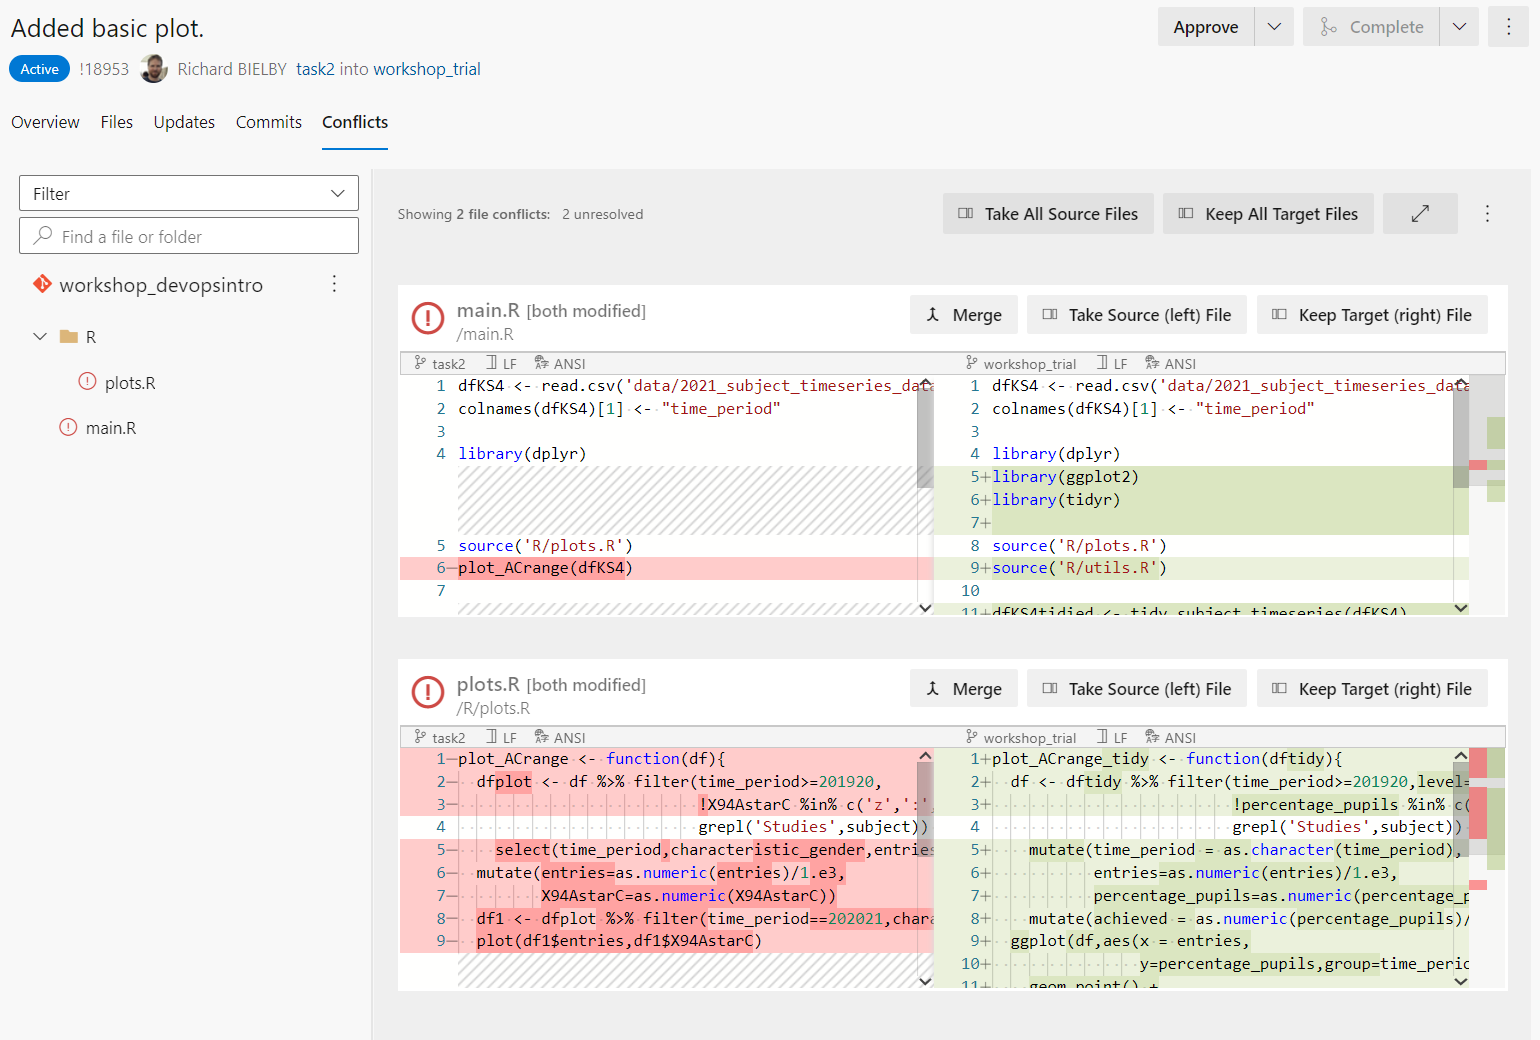
\includegraphics[width=0.96\linewidth]{images/DevOpsdemo/DevOps_PR_mergeconflict_1} 

}

\caption{Staging files in the RStudio git panel.}\label{fig:unnamed-chunk-17}
\end{figure}

You've got three options for resolving the conflict: \textbf{Merge},
\textbf{Take Source (left) file} and \textbf{Take Target (right) file}.
For a simple conflict where just one or the other version is appropriate
then you can click the corresponding of the latter two options. Here we
have something a little more complicated, so we want to go in and edit
and re-arrange the code ourselves. Click \textbf{Merge} and you'll get a
new screen showing the two versions side by side with an editor panel
below.

For the \texttt{main.R} file, change the conflicting lines in the editor
to be the following and then click \textbf{Submit merge}.

\begin{verbatim}
   library(dplyr)
   library(ggplot2)
   library(tidyr)

   source('R/plots.R')
   source('R/utils.R')

   plot_ACrange(dfKS4)

   dfKS4tidied <- tidy_subject_timeseries(dfKS4)
   plot_ACrange_tidy(dfKS4tidied)
\end{verbatim}

And for the \texttt{plots.R} file, simply remove the
\textbf{auto-generated} lines in the editor (you might also get asked to
add a line ending, in which case choose \emph{LF}) and again click
\textbf{Submit merge}.

Back on the Overview page, it should now say \emph{No merge conflicts}
and the \textbf{Complete} button should be available to click. Now the
PR is ready for your collaborators to review and approve and then you
can complete the PR and merge into your group's workshop branch.

Once you've completed the PR, head back to the team board on Dev Ops and
open up the task 2. You'll now see that the PR is listed under the
Devlopement section on the right as completed. To mark the task as
finished, close the task dialogue box and drag the task from Active to
Closed.

\hypertarget{notes-on-reviewing-a-pull-request}{%
\subsubsection{Notes on reviewing a pull
request}\label{notes-on-reviewing-a-pull-request}}

There are some basic steps to go through if you're asked to review a
pull request. The key elements are:

\begin{enumerate}
\def\labelenumi{\arabic{enumi}.}
\tightlist
\item
  Review any automated checks or QA scripts;
\item
  Clone the repository, switch to the relevant branch and run the code;
\item
  Look through and comment on the changes to the repository using the
  \textbf{Files changes} panel in the PR.
\end{enumerate}

In this case, we don't have any automated checks set up properly, so
we'll focus on points 2 and 3.

First of all try switching to the \emph{featTimeSeriesChart} branch if
you're not already in it and run the Shiny app - this can be done by
opening the global.R script in RStudio and clicking Run App in the top
right hand corner of the viewer pane. Assuming the dashboard runs, then
try cycling through the different panels of the dashboard looking for
any problems, errors or just things that could be improved.

There should be plenty of issues to find as we've kept the actual
dashboard coding brief to focus on using git. As you find them, enter
them in to the GitHub pull request, either under \textbf{Review changes}
on the Files changed panel or as comments in the \textbf{Conversation}
panel.

In reality, once you've got those reviews collated, you'd go through and
make changes to the code accordingly. This provides the checks and
balances and a structure for code QA necessary when developing
reproducible analyticle pipelines or data dashboards.

Assuming we've dealt with the outcomes of those reviews appropriately,
the next step is to complete the Pull request by clicking the
\textbf{Merge pull request} button. This then completes the merge in to
\emph{main} in this case. Whilst the basic mechanics of what's happening
with the branches is the same here as with just running
\texttt{git\ merge}, the Pull request provides that extra layer of
administrative structure to perform proper QA of the code and the
resulting product.

\hypertarget{summary-1}{%
\subsection{Summary}\label{summary-1}}

We've looked through a lot of the basics in this section, covering
adding/staging, committing, pushing/pulling between remote and local
repos, merging and pull requests. These are all the main concepts you
need to use git.

We've also tried to cover doing all this through a mixture of RStudio,
git BASH and GitHub (and as we've said Azure Dev Ops offers similar
functionality to GitHub). Most common processes can be done multiple
ways and there's not necessarily a single right method to follow, just
whichever makes most sense in your situation.

Just a quick final note on why it's useful to be familiar with git
\texttt{BASH}. Whilst most of the basic git functionality can be
accessed via the RStudio panel or GitHub/Dev Ops, there are some things
that are best achieved through BASH. In particular, if you have a file
in your repo that you need to remove entirely, this pretty much requires
someone to use commands via git BASH.

\begin{longtable}[]{@{}
  >{\raggedright\arraybackslash}p{(\columnwidth - 4\tabcolsep) * \real{0.2113}}
  >{\raggedright\arraybackslash}p{(\columnwidth - 4\tabcolsep) * \real{0.4225}}
  >{\centering\arraybackslash}p{(\columnwidth - 4\tabcolsep) * \real{0.3662}}@{}}
\toprule()
\begin{minipage}[b]{\linewidth}\raggedright
Process
\end{minipage} & \begin{minipage}[b]{\linewidth}\raggedright
git BASH
\end{minipage} & \begin{minipage}[b]{\linewidth}\centering
RStudio git panel
\end{minipage} \\
\midrule()
\endhead
Create branch & \texttt{git\ checkout\ -b\ branch\_name} &
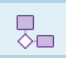
\includegraphics{"images/gitdemo/gitdemo-RStudio-gitToolbarCreateBranch.png"} \\
Switch branch & \texttt{git\ checkout\ branch\_name} &

\includegraphics{"images/gitdemo/gitdemo-RStudio-gitToolbarSwitchBranch.png"} \\
Merge branch & \texttt{git\ merge\ branch\_name} & N/A - use GitHub/Dev
Ops \\
\bottomrule()
\end{longtable}

\newpage

\hypertarget{troubleshooting}{%
\section{Troubleshooting}\label{troubleshooting}}

\hypertarget{renv}{%
\subsection{renv}\label{renv}}

If \texttt{renv::restore()} causes issues, then one of your team should
try \texttt{renv::init()} and select option 2 to restart renv. Then do a
add/commit/push cycle and get the other team members to do a pull and
then try running \texttt{renv::restore()} again on their local clones of
the repo.

\hypertarget{datafiles-commit-hooks.gitignore}{%
\subsection{\texorpdfstring{Datafiles
commit-hooks/\texttt{.gitignore}}{Datafiles commit-hooks/.gitignore}}\label{datafiles-commit-hooks.gitignore}}

To help teams keep on top of avoiding any accidental publishing of
unpublished data, we've added in some code around commits that checks
through any data files in the repo and checks them against a logfile and
the .gitignore file. Any files listed in .gitignore will not be included
in commits and therefore won't be sent to the remote repo as part of any
push.

\hypertarget{merge-conflicts}{%
\subsection{merge conflicts}\label{merge-conflicts}}

Merge commits happen when two branches have conflicting changes that
have been made concurrently. \texttt{git} can usually figure out how to
prioritise changes based on the commit history, but if changes have
happened at the same time to the same bit of code across different
branches, then it will need to get your input on how to prioritise the
changes.

The easiest way to go through how to deal with merge conflicts is by
discussing with an example, so ask us in the workshop if and when you
hit a merge conflict.

Briefly though, when there's a merge conflict, git will add some text to
the file containing the conflict along the following lines:

\begin{verbatim}
<<<<<<<<<<< branch_1
code 
on 
branch 
1
===========
conflicting code on branch 2
>>>>>>>>>>> branch_2
\end{verbatim}

Effectively as the user, you need to decide which bit of code is the
right bit to keep and then delete anything you don't want to keep as
well as the tag-lines that git has added in. So for example, you should
be left with something along the lines of:

\begin{verbatim}
code 
on 
branch 
1
\end{verbatim}

Once you've cleared up all merge conflicts in the branch that you're
working on, then perform another add/commit cycle and thay should clear
out the conflict from the branch that you're working on and you'll be
able to continue with the intended merge/PR.

\newpage

\resizebox{48mm}{!}{
\includegraphics{images/Department_for_Education.png}}
\vspace*{\fill}
\color{black}

© Crown copyright 2022

This publication (not including logos) is licensed under the terms of
the Open Government Licence v3.0 except where otherwise stated. Where we
have identified any third party copyright information you will need to
obtain permission from the copyright holders concerned.

To view this licence:

\begin{tabular}{p{0.02\linewidth} p{0.1\linewidth} p{0.88\linewidth}}
& visit & www.nationalarchives.gov.uk/doc/open-government-licence/version/3 \\
& email & psi@nationalarchives.gsi.gov.uk \\
& write to & Information Policy Team, The National Archives, Kew, London, TW9 4DU \\
\end{tabular}

About this publication:

\begin{tabular}{p{0.02\linewidth} p{0.1\linewidth} p{0.88\linewidth}}
& enquiries & www.education.gov.uk/contactus \\
& download & www.gov.uk/government/publications \\
\end{tabular}

\begin{tabular}[t]{p{0.06\linewidth} p{0.24\linewidth} p{0.04\linewidth} p{0.06\linewidth} p{0.36\linewidth}}
\raisebox{-.5\height}{
\includegraphics{images/logoTwitter.png}} &
Follow us on Twitter: @educationgovuk &
&
\raisebox{-.5\height}{
\includegraphics{images/logoFacebook.png}} &
Like us on Facebook: \qquad facebook.com/educationgovuk\\
\end{tabular}

\end{document}
